%====================================================================%
%                  MORIOND.TEX                                       %
%====================================================================%

\documentclass{moriond}


\bibliographystyle{unsrt}    
% for BibTeX - sorted numerical labels by order of
% first citation.

% A useful Journal macro
\def\Journal#1#2#3#4{{#1} {\bf #2}, #3 (#4)}

% Some useful journal names
\def\NCA{\em Nuovo Cimento}
\def\NIM{\em Nucl. Instrum. Methods}
\def\NIMA{{\em Nucl. Instrum. Methods} A}
\def\NPB{{\em Nucl. Phys.} B}
\def\PLB{{\em Phys. Lett.}  B}
\def\PRL{\em Phys. Rev. Lett.}
\def\PRD{{\em Phys. Rev.} D}
\def\ZPC{{\em Z. Phys.} C}
\def\JINST{\em JINST}
\def\JHEP{\em JHEP}
\def\EPJC{\em EPJC}

% Some other macros used in the sample text
\def\st{\scriptstyle}
\def\sst{\scriptscriptstyle}
\def\mco{\multicolumn}
\def\epp{\epsilon^{\prime}}
\def\vep{\varepsilon}
\def\mt{m_{\textrm{T}}}
\def\et{E_\textrm{T}^{\textrm{miss}}}
\def\ptmiss{\vec{p}_\textrm{T}^{\textrm{miss}}}
\def\ra{\rightarrow}
\def\ppg{\pi^+\pi^-\gamma}
\def\vp{{\bf p}}
\def\pt{{p_{\textrm{T}}}}
\def\ko{K^0}
\def\kb{\bar{K^0}}
\def\al{\alpha}
\def\ab{\bar{\alpha}}
\def\be{\begin{equation}}
\def\ee{\end{equation}}
\def\bea{\begin{eqnarray}}
\def\eea{\end{eqnarray}}
\def\CPbar{\hbox{{\rm CP}\hskip-1.80em{/}}}
%temp replacement due to no font
%%%%%%%%%%%%%%%%%%%%%%%%%%%%%%%%%%%%%%%%%%%%%%%%%%
%                                                %
%    BEGINNING OF TEXT                           %
%                                                %
%%%%%%%%%%%%%%%%%%%%%%%%%%%%%%%%%%%%%%%%%%%%%%%%%%

\begin{document}
\vspace*{0cm}
\title{Searches for exotic Dark Matter at ATLAS and CMS}


\author{Bingxuan Liu, on behalf of the ATLAS and CMS Collaborations}

\address{Department of Physics, Simon Fraser University, Vancouver, Canada}

\maketitle\abstracts{The nature of dark matter is still a mystery. Many direct
and indirect search experiments are trying to solve this puzzle. The LHC offers
a unique opportunity at the high energy frontier, where dark matter particles
or related new particles may be produced and detected. Both the CMS and ATLAS
collaborations have carried out comprehensive dark matter search programs,
providing critical experiemntal results. In this article, recent exotic dark
matter searches in CMS and ATLAS are summarized and a brief outlook is given.}

\section{Introduction}

The nature of DM remains a mystery and there are many Beyond Standard Model
(BSM) theories proposed to offer an explanation. LHC~\cite{LHCRef} offers a
unique opportunity to search for Dark Matter (DM) and related new particles at
the high energy frontier.  ATLAS~\cite{ATLASRef} and CMS~\cite{CMSRef} are the
two general-purpose detectors at the LHC that are capable of searching for new
particles using a rich set of signatures. Both experiments have carried out
comprehensive dedicated DM search programs, primarily in the following
categories: 

\begin{itemize}
\item Mono-X Signature: DM candidates are produced in association with another detectable physics object (X). The non-interacting DM candidates give rise to a sizable missing transverse energy ($\et$). The detectable physics object can be a jet, photon, $Z$ boson and Higgs boson, or a Beyond Standard Model (BSM) particle that decays visibly.   
\item Resonance Signature: The mediator coupled to DM candidates is produced resonantly, decaying to SM particles to form a peak in the invariant mass spectrum. The SM pariticles can be a pair of jets, leptons or bosons. 
\item Associated Production with Heavy Flavor Quarks: DM candidates are produced in association with heavy flavor quarks, including a single top quark or a pair of top/bottom quarks. 
\item Supersymmetry (SUSY) Searches: DM candidates are produced in certain SUSY models which usually features a high jet multiplicity final state with a significant $\et$.  
\item SM Higgs Portal: DM candidates are decay products of the Higgs boson, where the Higgs boson is produced via SM processes. There is a sizable $\et$ recoiled against the visible physics objects which depends on the production mode of the Higgs boson such as the vecotr boson fusion (VBF). 
\end{itemize}    

The DM search program is expanding. The full LHC Run 2 data brings higher
precision to inclusive DM searches such as the mono-jet, mono-$Z$ and
mono-Higgs searches. More final states are being explored with aid from
innovative analysis techniques such as VBF + $\et$\ +
$\gamma$ and mono-s($\rightarrow VV$), motivated by theories such as dark
Higgs~\cite{DarkH} and dark photon~\cite{DarkPh}. In the meantime, the
theoretical framework has also advanced in the past decades, taking the
experiment results into account.  As a consequence, more models have thrived,
encouraging both CMS and ATLAS to provide more interpretations. In paricular,
the 2HDM+a model~\cite{2HDM} is widely considered in recent searches.
Figure~\ref{fig:diagrams} shows the diagrams of the models mentioned a bove.

\begin{figure} [htb]
\begin{minipage}{0.32\linewidth}
\centerline{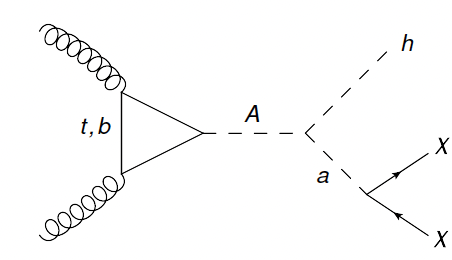
\includegraphics[width=0.9\linewidth]{2HDM_a}}
\end{minipage}
\begin{minipage}{0.32\linewidth}
\centerline{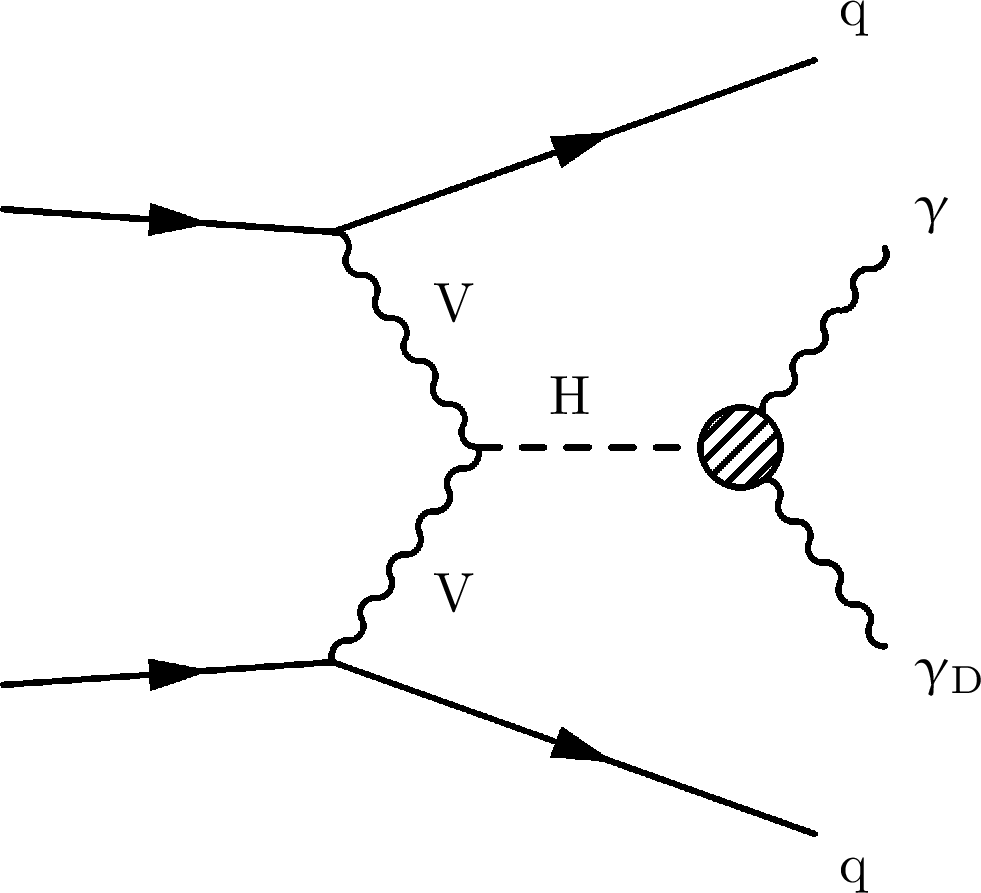
\includegraphics[width=0.9\linewidth]{HiggsDarkPhotonDiagram}}
\end{minipage}
\begin{minipage}{0.32\linewidth}
\centerline{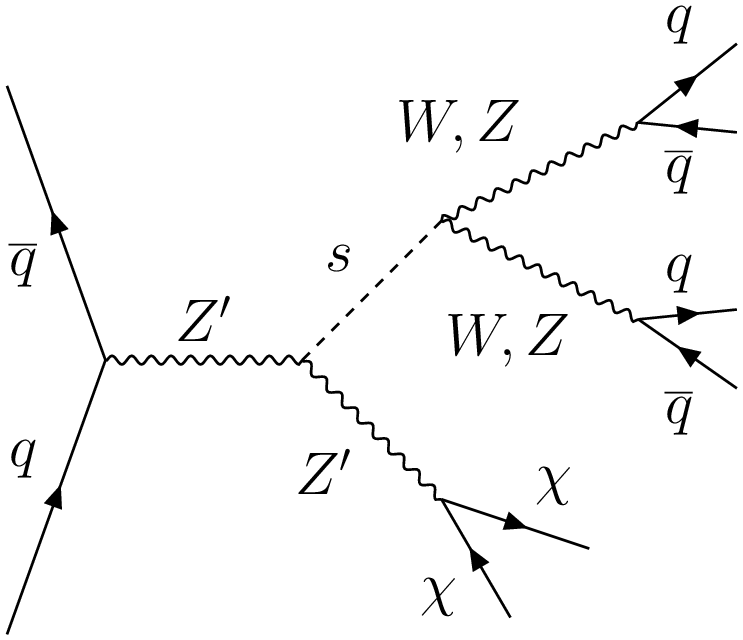
\includegraphics[width=0.9\linewidth]{MonoSVVDiagram}}
\end{minipage}
\caption[]{Diagrams of various models considered in recent DM searches. Left: A Higgs boson is produced in association with a pseudo-scalar decaying to DM candidates (2HDM+a); middle: a Higgs boson is produced in the VHF channel, decaying to a photon and a dark photon; right: a dark Higgs s is produced in association with a $Z/pime$, where the $Z/prime$ decays to DM candidates and the dark higgs s decays to two vectro bosons.}
\label{fig:diagrams}
\end{figure}

Recent results from both CMS and ATLAS will be summarized in the next section
followed by an outlook on the future DM seearch programs at the LHC. All
searches discussed in this article use full Run 2 dataset. 

\section{Dedicated search results}

\subsection{Mono-X searches}

Mono-jet search is the flagship analysis in the DM regime as its simple final
state covers a large range of parameter space, sensitive to many different
models. The recent ATLAS mono-jet search~\cite{monojet} uses data collected by a $\et$\
trigger. The events are required to have at least one energetic jet and not
have leptons or photons present. Signal regions are divided by $\et$\.

Mono-$Z$ is also a very important inclusive search. The recent CMS mono-$Z$
search~\cite{monoz} considers the leptonic final state where the $Z$ boson
decays to either a pair of muons or electrons. Events are collected by dimuon
(dielectron) triggers and must contain two well-identified, isolated muons
(electrons) with the same flavor and opposite charge, forming an invariant mass
compatible with the $Z$ boson mass. Events with additioanl leptons, more than
one jet or any $b$-tagged jets are vetoed to supress the backgrounds. Signal
regions are constructed based on either the missing transverse momentum,
$\ptmiss$, or the transverse mass between the di-lepton system and $\ptmiss$,
$\mt$. The latter one is optimized for 2HDM+a model as there is a peak in $\mt$
spectrum near the neutral scalar (H) mass. 

\begin{figure} [htb]
\begin{minipage}{0.45\linewidth}
\centerline{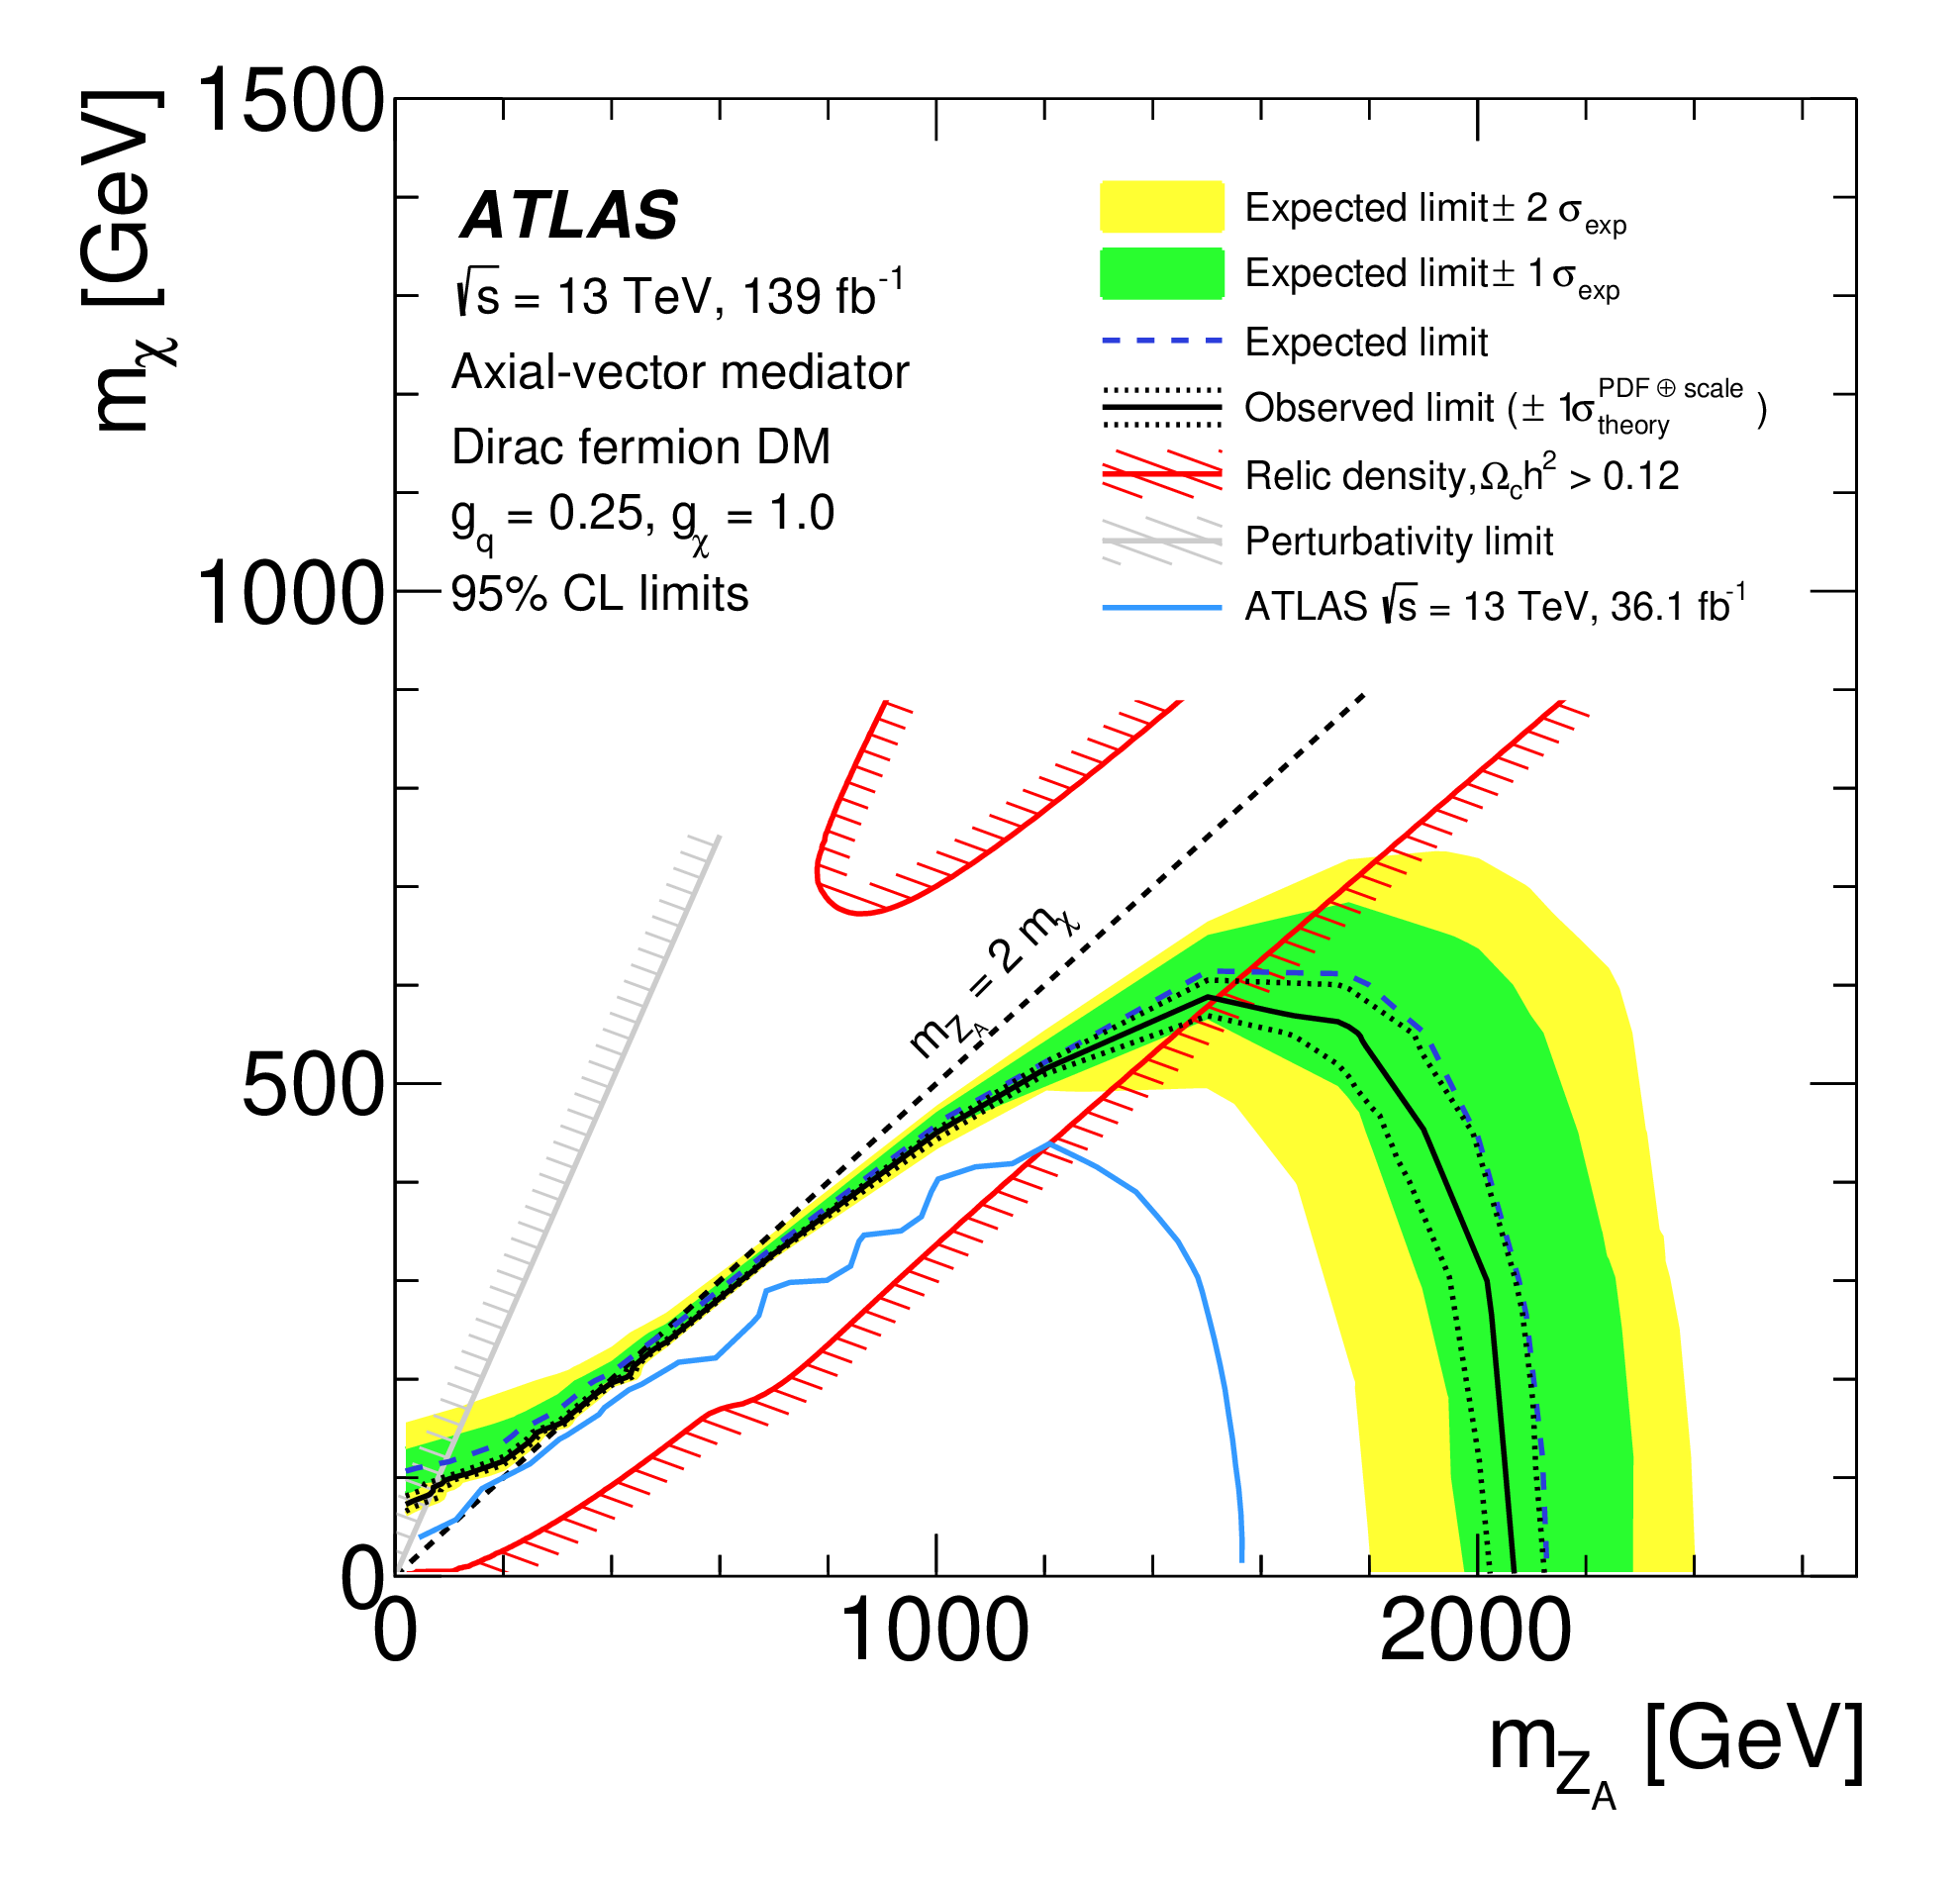
\includegraphics[width=0.9\linewidth]{monojet}}
\end{minipage}
\begin{minipage}{0.45\linewidth}
\centerline{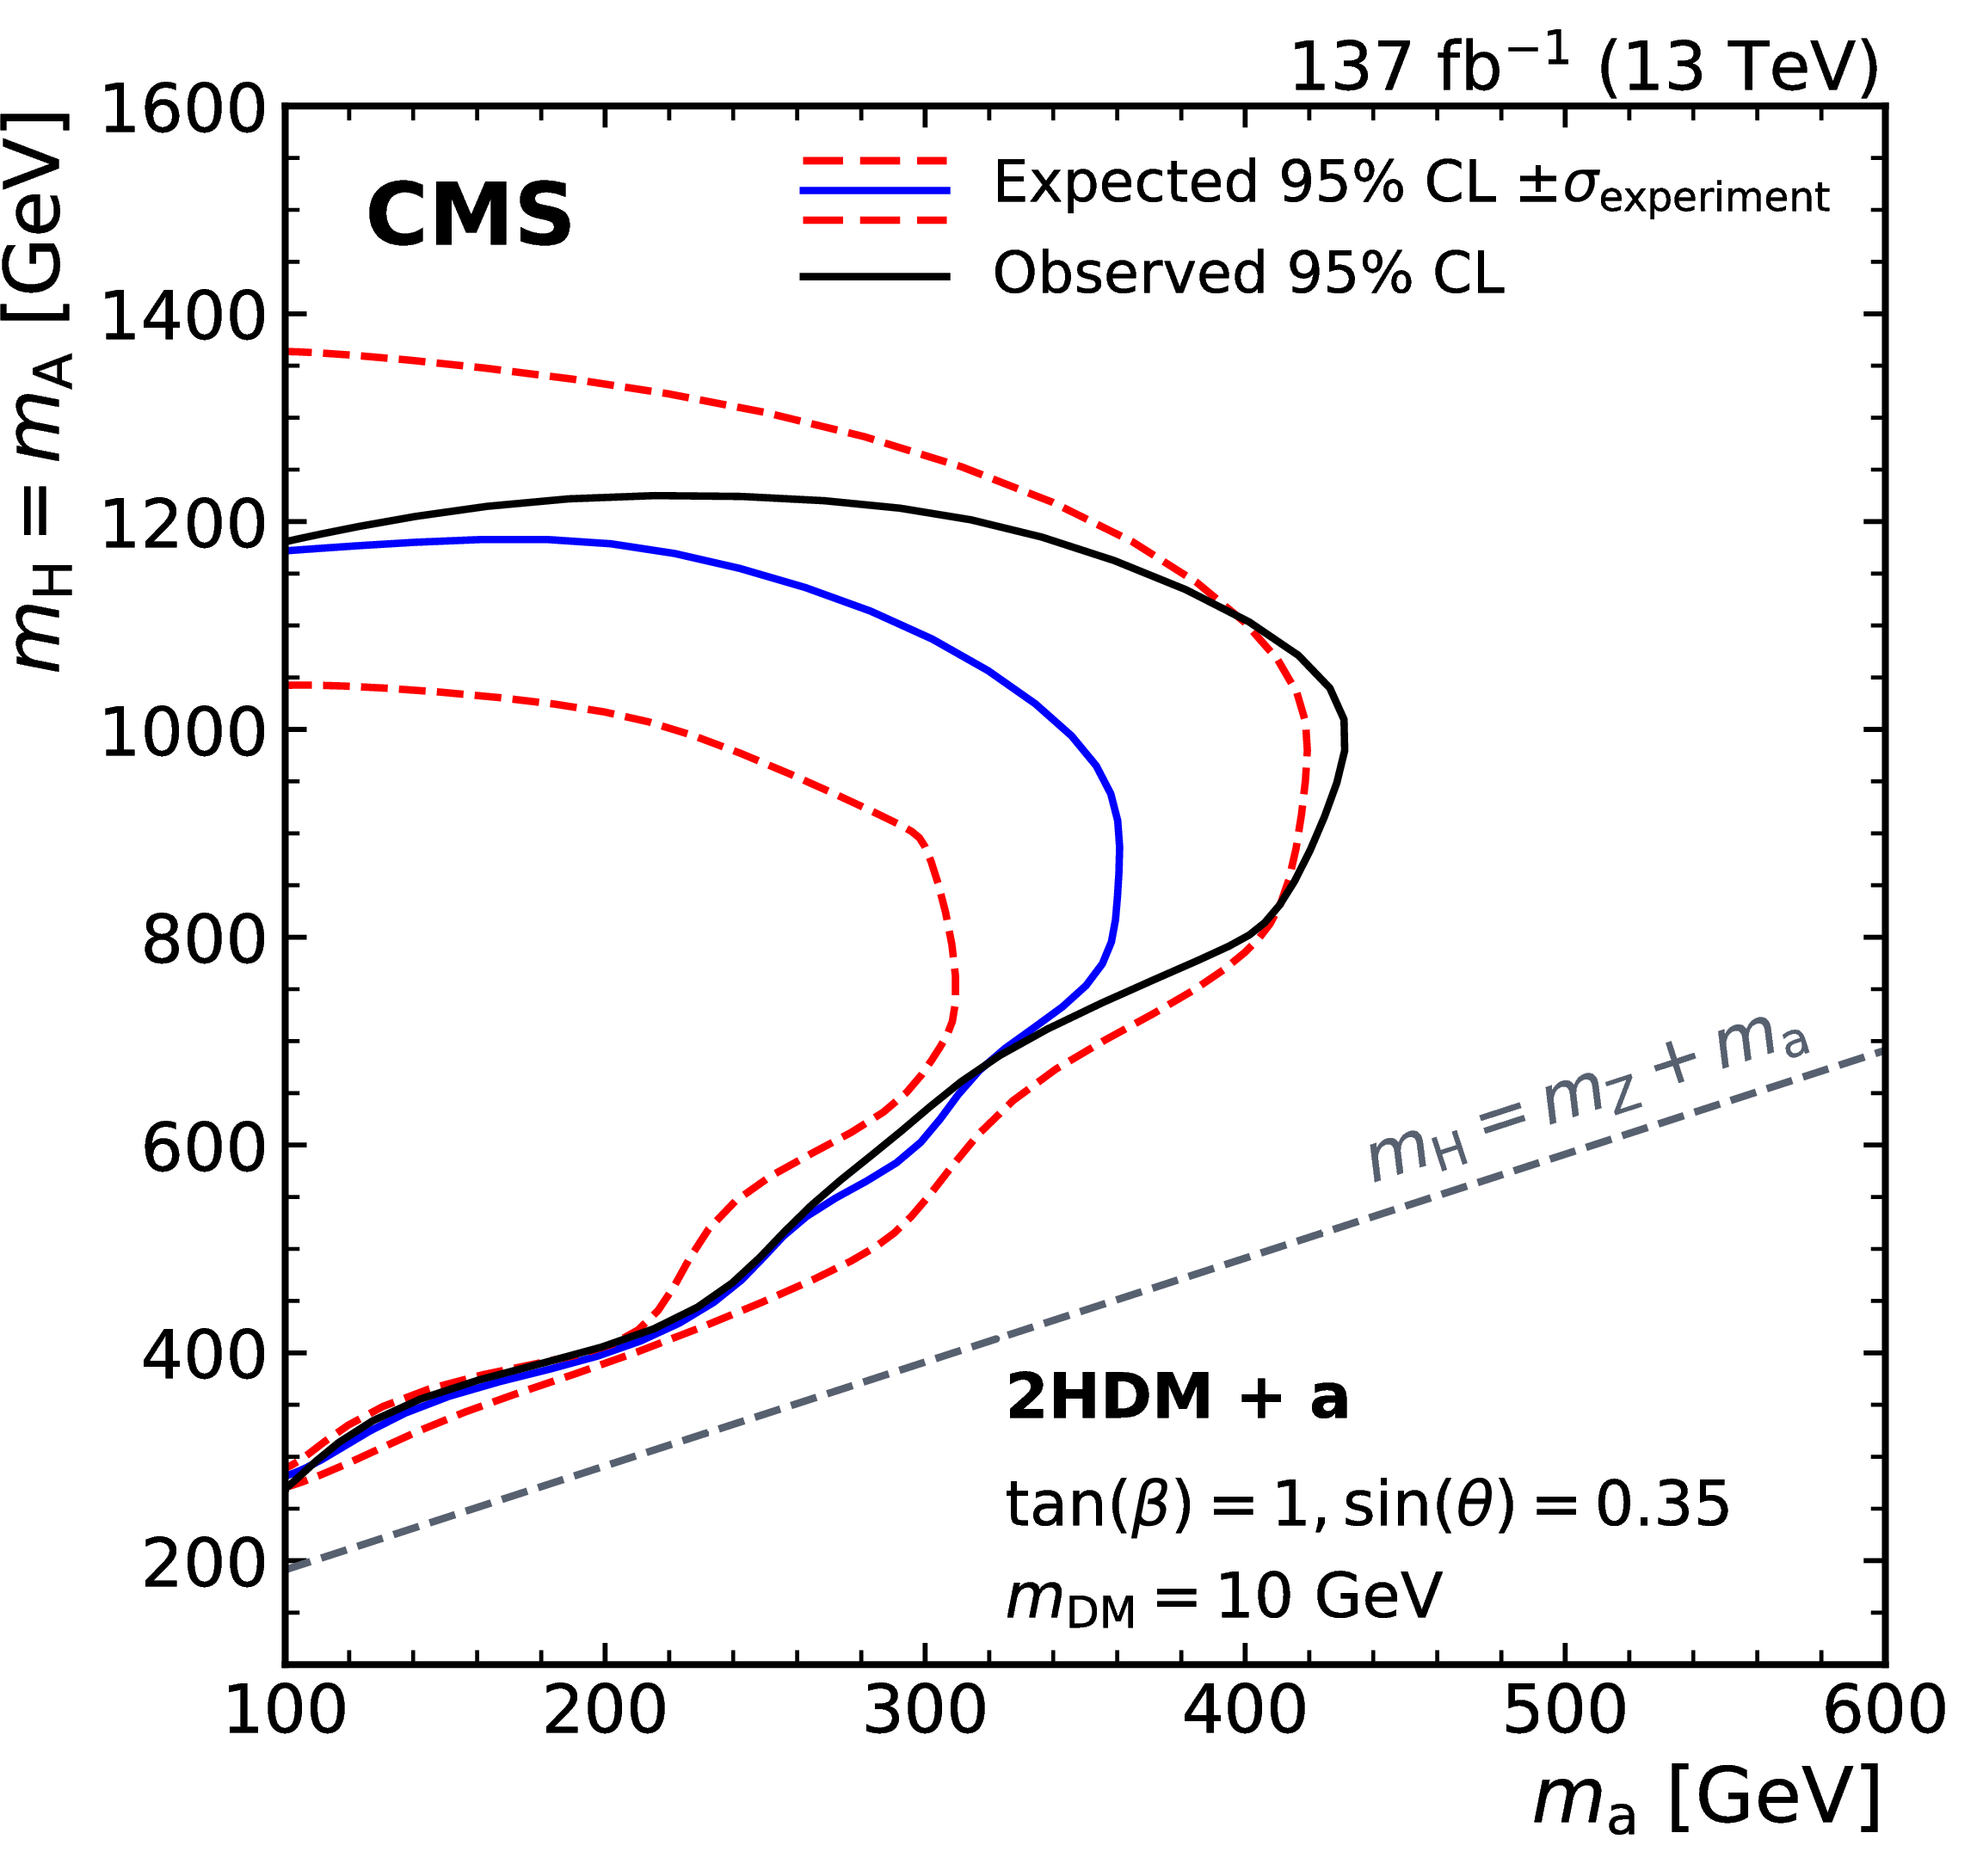
\includegraphics[width=0.9\linewidth]{monoz}}
\end{minipage}
\caption[]{}
\label{fig:mono_jet_z}
\end{figure}

Both the mono-jet and mono-$Z$ search considers well know detectable standard
model (SM) physic objects. Searches considering less well known SM particles
such as the Higgs boson or new BSM particles such as a new scalar target the
specific phase space, facing different experimental challenges. The recent
ATLAS mono-Higgs($\rightarrow b\overline{b}$) search~\cite{monoh} considers
events collected by the primary $\et$\ triggers. Events are required to have
sizable $\et$\ and veto isolated leptons. The signal regions are categorized by
the $b$-tagged multiplicity (two or three) and the collinearity of the two
$b$-tagged jets forming the Higgs candidate (merged and resolved). The ATLAS
mono-s($\rightarrow VV$) search~\cite{monos} probes a similar final states with
sizable $\et$\ but looks for hadronic boson decays instead of $b$-hadron
decays. Events must contain two boson tagged jets, and the signal regions are
categorized by their collinearity (merged and intermediate).    

\begin{figure} [htb]
\begin{minipage}{0.45\linewidth}
\centerline{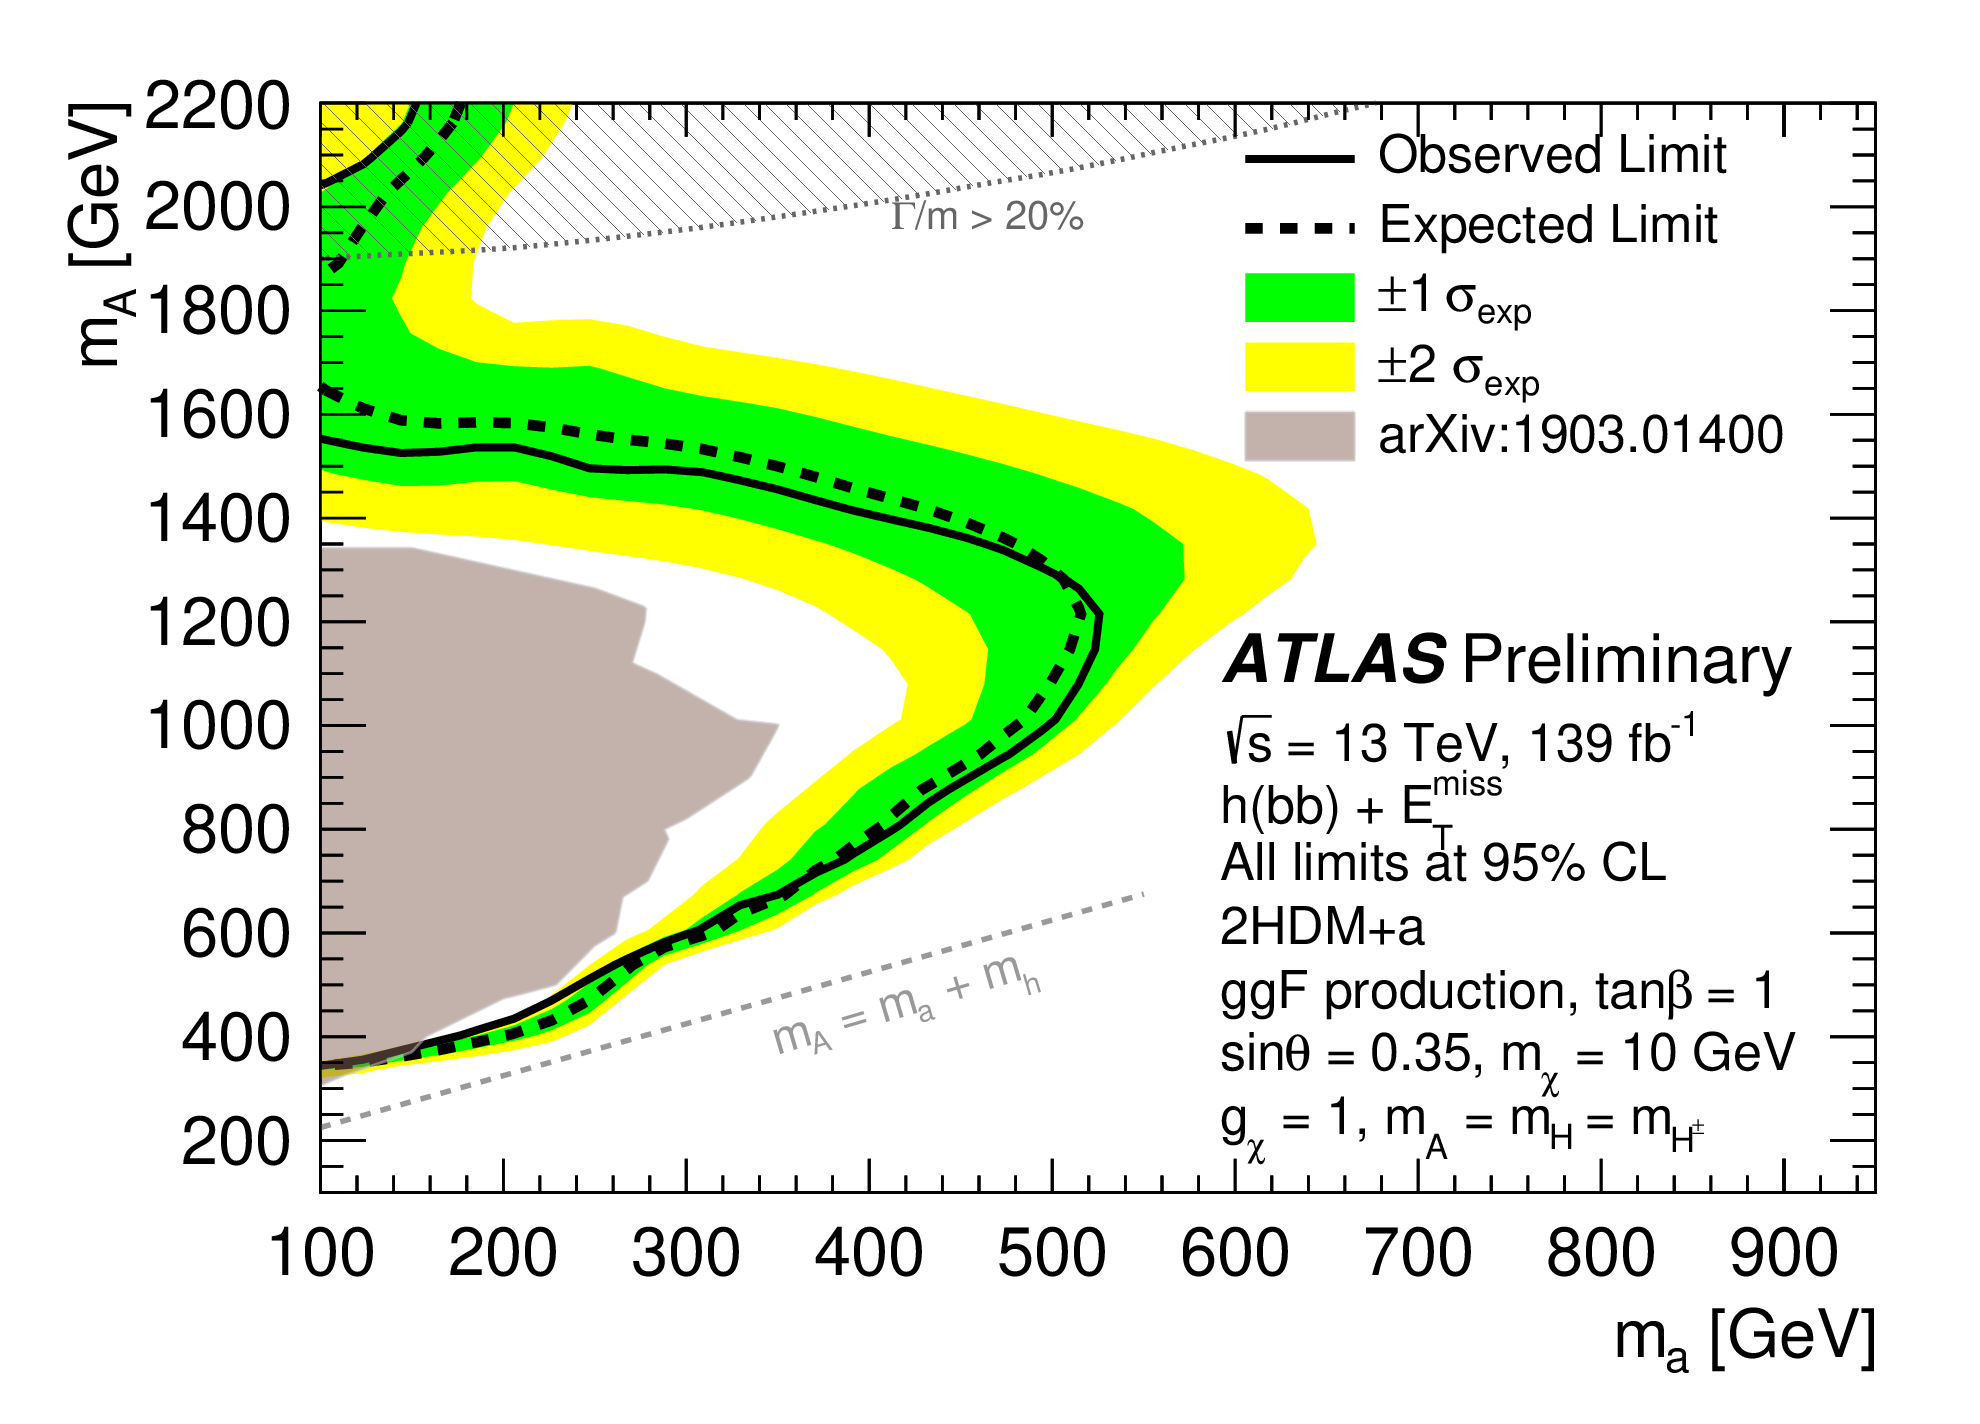
\includegraphics[width=0.9\linewidth]{monoh}}
\end{minipage}
\begin{minipage}{0.45\linewidth}
\centerline{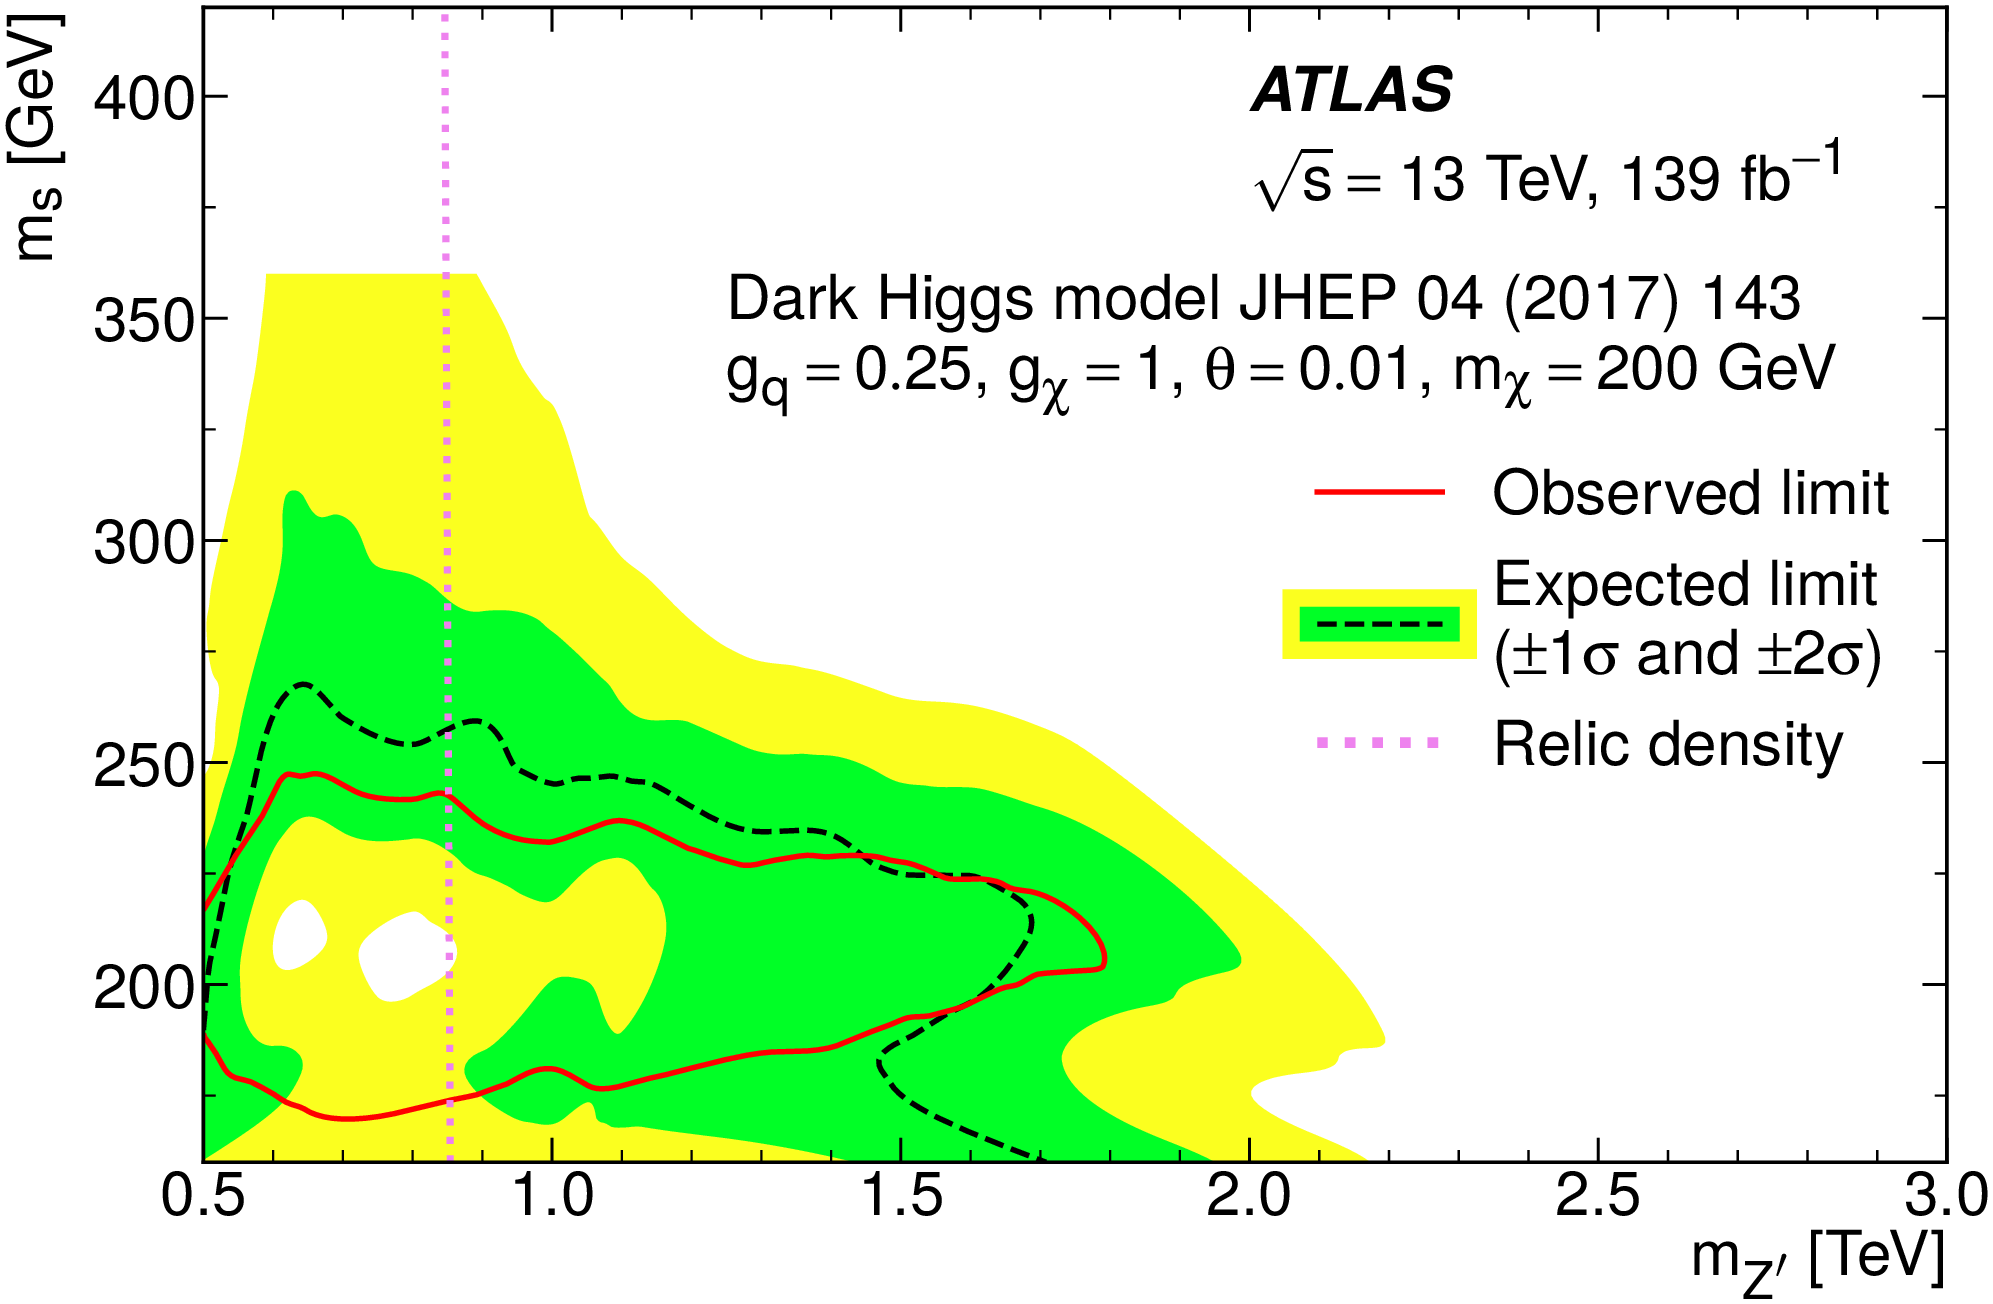
\includegraphics[width=0.9\linewidth]{monos}}
\end{minipage}
\caption[]{}
\label{fig:mono_h_s}
\end{figure}

\subsection{Dark photon search in the VBF channel}

As the most recently discovered SM particle, the Higgs boson opens up an
interesting avenue for DM search, not only because it can be produced in
association with DM particles but also it can decay to DM particles. The
Higgs$\rightarrow inv$) branching ratio is a critical channel to study the
phase space where $m_{i\textrm{DM}} < \frac{1}{2}m_{\textrm{H}}$. The combined
Higgs$\rightarrow inv$ branching ratio measurement~\cite{hiv} sets a stringent
upper limit of 0.11 at 95\% CL. Recent ATLAS~\cite{atlasvbf} and
CMS~\cite{cmsvbf} searches explored another unique scenario where the Higgs
decays to a dark photon and a photon, which gives sizable $\et$\ and a photon
in the final state. Both searches consider the VBF production channel given its
larger cross section, applying similar event selections such as containing VBF
jets and lepton veto. The $\mt$\ between the photon and the $\ptmiss$\ is used
as the discriminat variable to categorize the signal regions. It is worth
mentioning that ATLAS applies a lower photon $p_{\textrm{T}}$ threshold and
additional jet centrality cuts to achieve better stronger exclusion limits.  

\begin{figure} [htb]
\begin{minipage}{0.45\linewidth}
\centerline{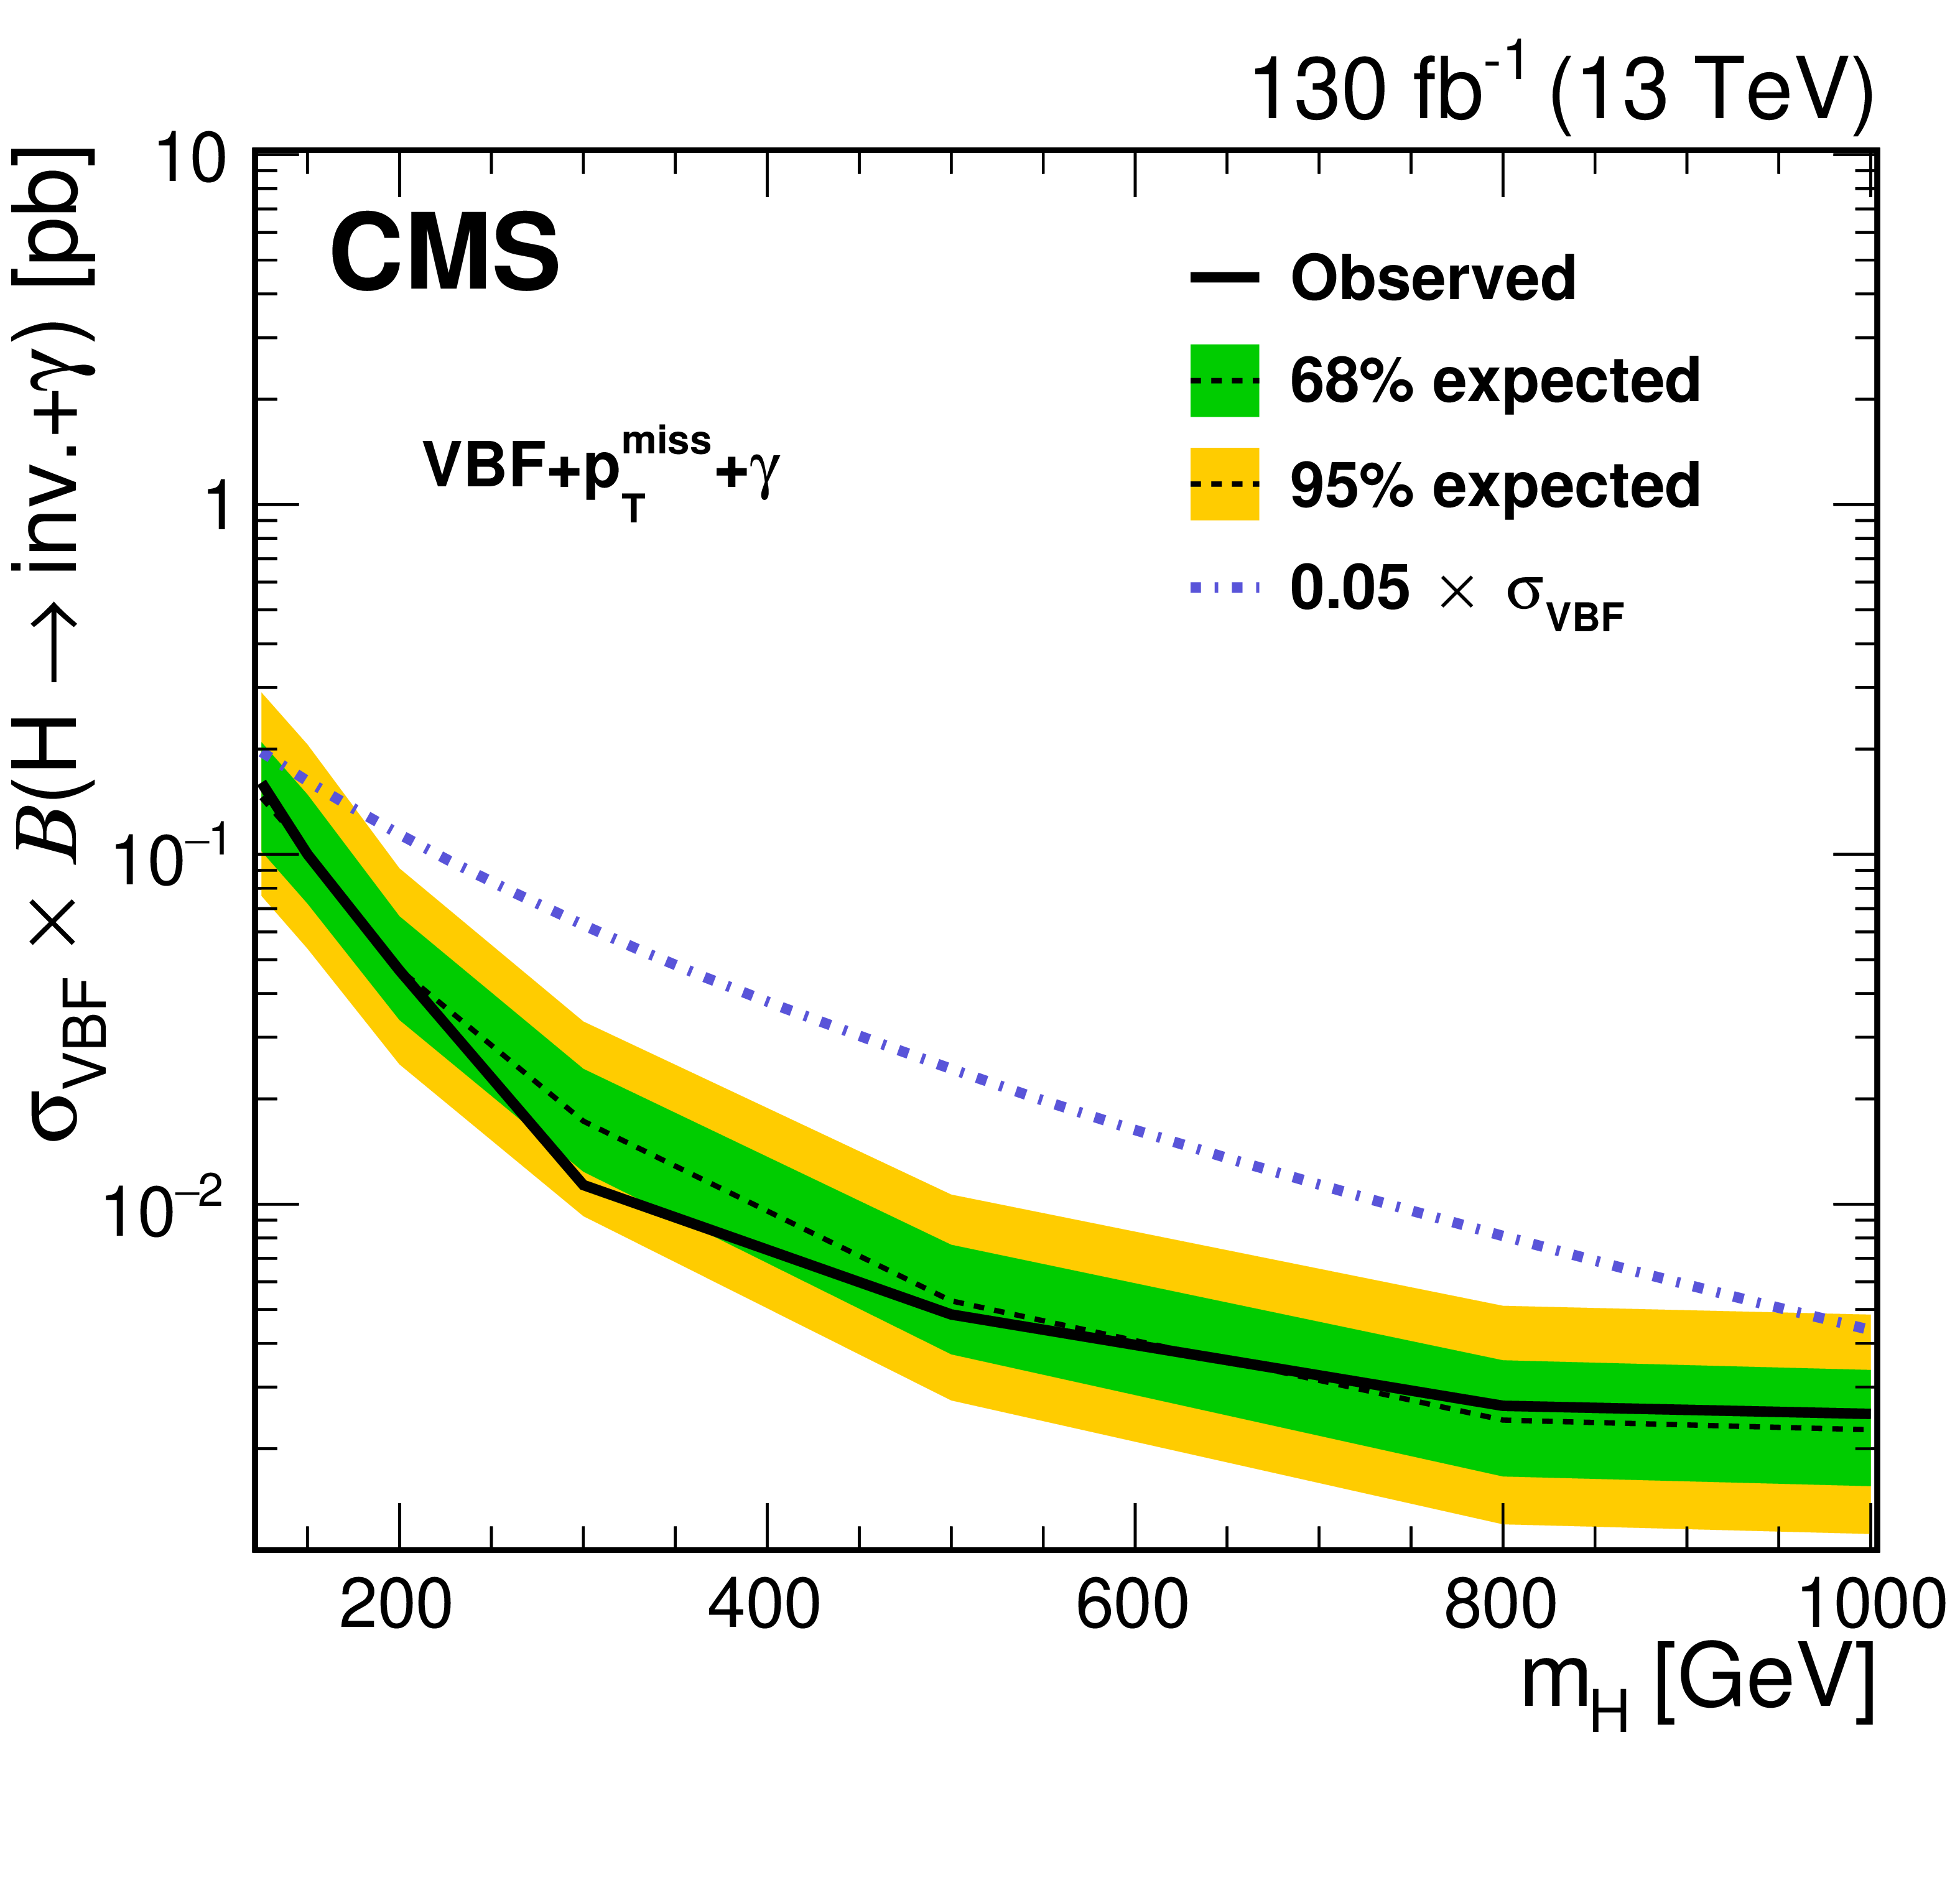
\includegraphics[width=0.9\linewidth]{cmsvbf}}
\end{minipage}
\begin{minipage}{0.45\linewidth}
\centerline{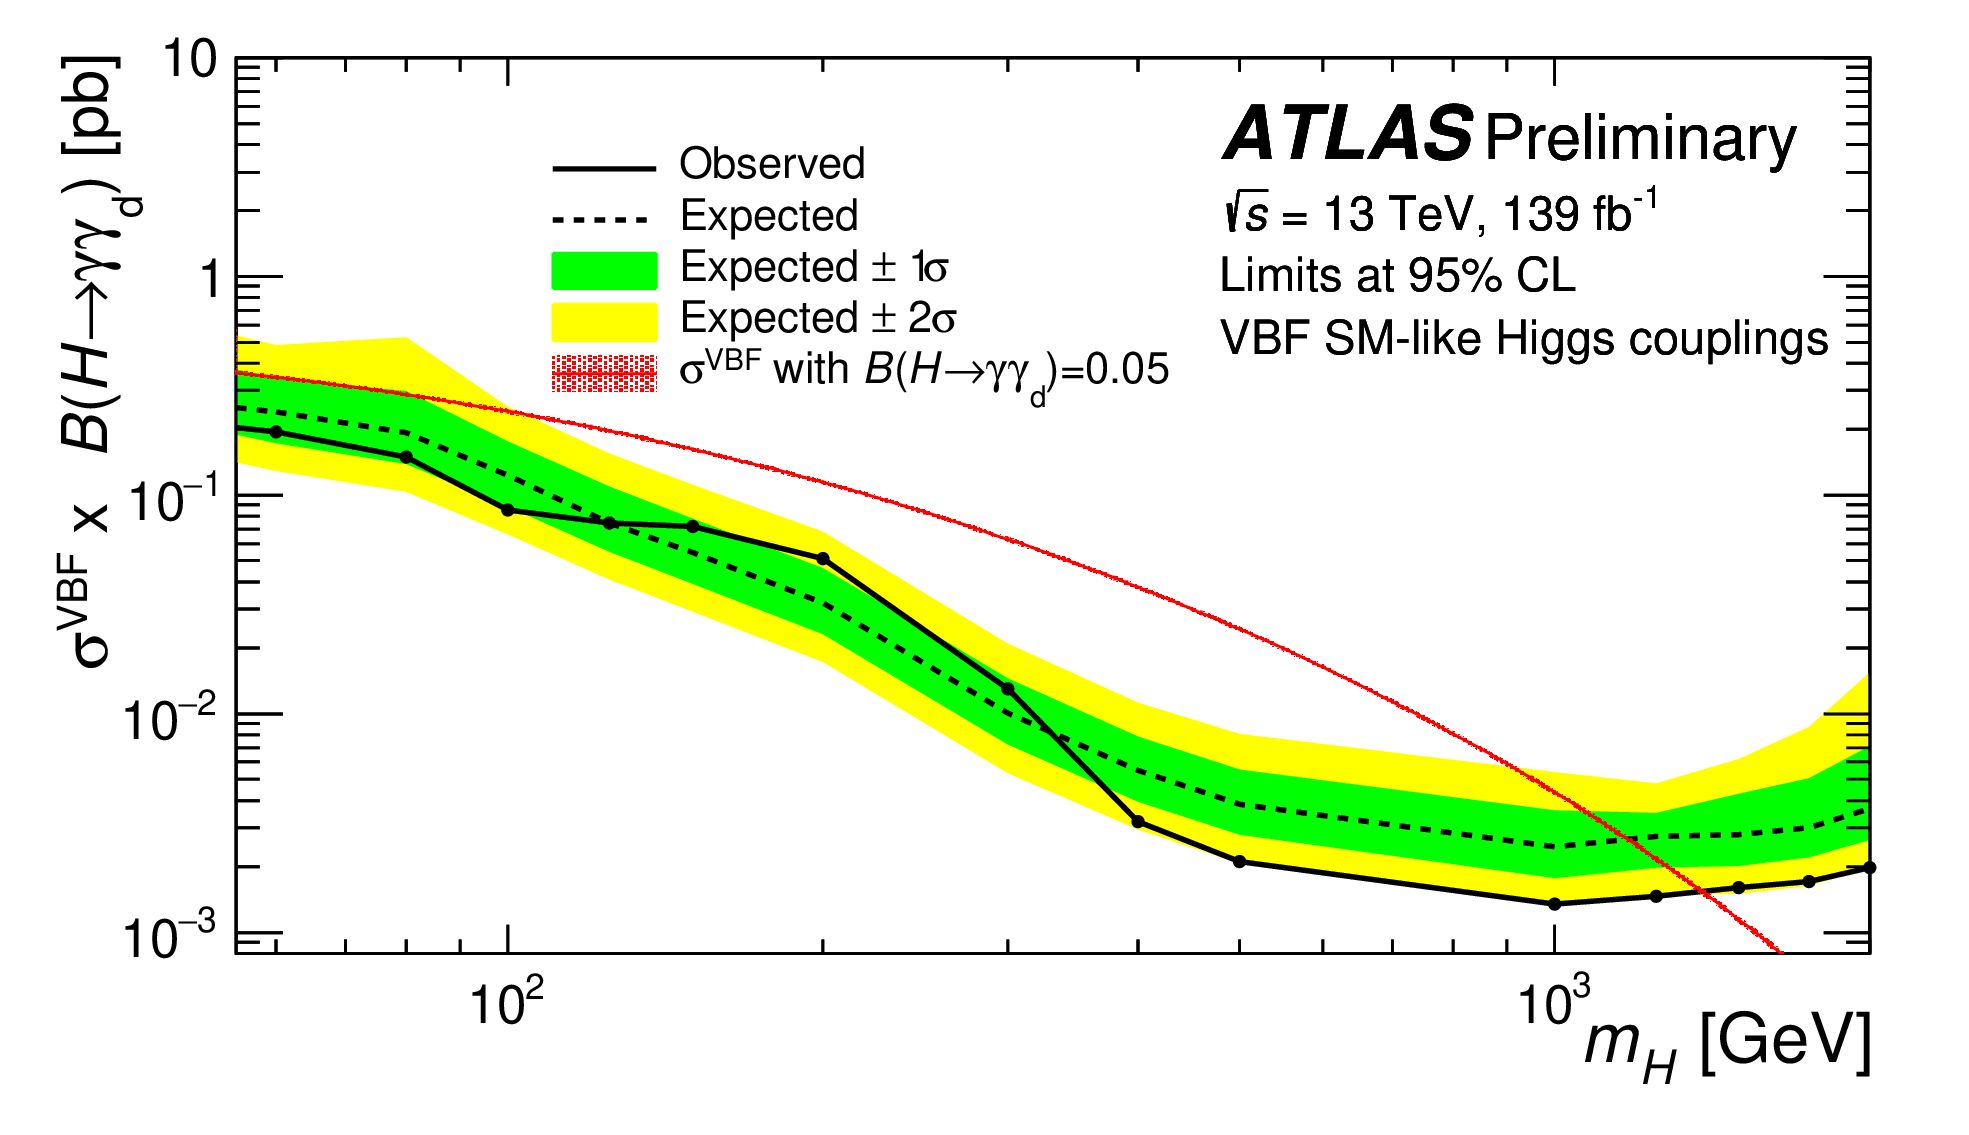
\includegraphics[width=0.9\linewidth]{atlasvbf}}
\end{minipage}
\caption[]{}
\label{fig:vbf}
\end{figure}

\subsection{DM interpretations in SUSY searches}

R-parity conserving (RPC) SUSY predicts a stable lightest supersymmetric
particle (LSP), which is a good DM candidate. SUSY searches targetting this
scenario usually requires large $\et$ and high jet ($b$-tagged jet)
multiplicity. Certain DM models may share similar final states. In a recent
ATLAS SUSY search~\cite{dmbb}, a dedicated signal region is constructed and
optimized for DM particles produced in association with a pair of $b$-quarks.      

\begin{figure} [htb]
\centerline{\includegraphics[width=0.5\linewidth]{DMBB}}
\caption[]{}
\label{fig:dmbb}
\end{figure}

\section{Conclusions}

LHC has explored a very large parameter space where DM could have existed.
Recent theoretical development encourages searches to look at more specific
final states in addition to the inclusive ones and several new results from
both CMS and ATLAS already extended the scope of the DM search program to new
horizons. There are still many ongoing full Run 2 DM searches that will further
broaden the coverage. The hunt is still on!

\section*{References}

\begin{thebibliography}{99}

\bibitem{LHCRef}L. Evans and P. Bryant (editors), \Journal{\JINST}{3}{S08001}{2008}.

\bibitem{CMSRef}CMS Collaboration, \Journal{\JINST}{3}{S08004}{2008}.

\bibitem{ATLASRef}ATLAS Collaboration, \Journal{\JINST}{3}{S08003}{2008}.

\bibitem{DarkH}Duerr, Michael and Grohsjean, Alexander and Kahlhoefer, Felix and Penning, Bjoern and Schmidt-Hoberg, Kai and Schwanenberger, Christian, \Journal{\JHEP}{04}{143}{2017}.

\bibitem{DarkPh}Biswas, Sanjoy and Gabrielli, Emidio and Heikinheimo, Matti and Mele, Barbara, \Journal{\PRD}{93}{093011}{2016}.

\bibitem{2HDM}Bauer, M., Haisch, U. and Kahlhoefer, F., \Journal{\JHEP}{05}{138}{2017}.

\bibitem{monojet}ATLAS Collaboration, CERN-EP-2020-238, https://cds.cern.ch/record/2752675.

\bibitem{monoz}CMS Collaboration, \Journal{\EPJC}{81}{13}{2021}.

\bibitem{monoh}ATLAS Collaboration, ATLAS-CONF-2021-006, http://cdsweb.cern.ch/record/2759211. 

\bibitem{monos}ATLAS Collaboration, \Journal{\PRL}{126}{121802}{2021} 

\bibitem{hinv}ATLAS Collaboration, ATLAS-CONF-2020-052, https://cds.cern.ch/record/2743055.

\bibitem{cmsvbf}CMS Collaboration, \Journal{\JHEP}{03}{011}{2021}.

\bibitem{atlasvbf}ATLAS Collaboration, ATLAS-CONF-2021-004, http://cdsweb.cern.ch/record/2758212.

\bibitem{dmbb}ATLAS Collaboration, CERN-EP-2021-001, https://cds.cern.ch/record/2750578.

\end{thebibliography}

\end{document}

%%%%%%%%%%%%%%%%%%%%%%
% End of moriond.tex  %
%%%%%%%%%%%%%%%%%%%%%%


%%% Local Variables: 
%%% mode: latex
%%% TeX-master: t
%%% End: 

%%% Local Variables: 
%%% mode: latex
%%% TeX-master: t
%%% End: 

%%% Local Variables: 
%%% mode: latex
%%% TeX-master: t
%%% End: 
